\documentclass[12pt]{article}
%\renewcommand\normalsize{\fontsize{10pt}{12pt}\selectfont}
\usepackage{graphicx} % Required for inserting images
\usepackage[left=2cm,right=2cm,top=2cm,bottom=1.5cm]{geometry}

\title{HW 8}
%\author{Dennis Wilkinson}
\date{due Tuesday April 29}

\begin{document}

\setlength{\parindent}{0pt}
\setlength{\parskip}{3mm}

FS1 Wilkinson HW 8, due Thursday June 5

\textbf{1.} There are rules for figuring out the current in series and parallel circuits. This problem walks you through how it works for a parallel circuit, as pictured below. Think of the resistors $R_1$ and $R_2$ as, say, appliances which are on and drawing current. 

\begin{figure}[h]
    \centering
    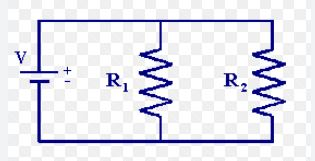
\includegraphics[width=0.3\linewidth]{parallel circuit.JPG}
\end{figure}

\textbf{a.} Let the current out of the battery be $I_{tot}$ Explain conceptually why there are two different currents, $I_1$ and $I_2$, going through $R_1$ and $R_2$ respectively, and why $I_1+I_2=I_{tot}$. 

\textbf{b.} Explain conceptually why the voltage \textit{across} $R_1$ (meaning, the difference in voltage between points in the wire on either side of $R_1$), and the voltage across $R_2$ both equal the battery voltage $V$.

\textbf{c.} Now we just have Ohm's Law on each resistor: $V=I_1R_1$ and similar for $R_2$. Rewrite $I_1+I_2=I_{tot}$ using these equations to find
\begin{equation}
I_{tot}=V\left( \frac{1}{R_1}+\frac{1}{R_2} \right).    
\end{equation}

\textbf{d.} In the case of a toaster ($R_1=12\Omega$) and a dishwasher when the pump and motor are on ($R_2=8\Omega$) plugged into $V=120$ volts, find $I_{tot}$, $I_1$ and $I_2$. (This is a simplification since in the household current is actually \textit{alternating}, which we haven't discussed, but just go with it for now.) 

\textbf{e.} Find the power supplied by the electric company, and the power used in each of the toaster and dishwasher, in the case of part (d).

\textbf{f.} If we turn another appliance on, we are (in some sense) adding resistance. So how is it that the total power supplied by the power company increases?

\textbf{g.} Now find $I_{tot}$ in the same arrangement, except replace the toaster with a short circuit - just a bare wire - that has a tiny resistance of $R_1=0.005 \Omega$. What happens in this case?

\textbf{h.} Explain why it would be a bad idea to put the toaster and the dishwasher in series, meaning, one after the other on the same branch of the circuit. Give two reasons.

\textbf{2*.} (non-calculus but hard - for y'all who have seen circuits before): Find the total current (out of the battery) in the following circuit. Answer: $\frac{19}{29}\frac{V}{R}$. Also, find the current in the middle resistor, and which way it's flowing. Hint: your variables are five different currents, one in each branch. I used conservation of charge at the junctions (two equations), and that the total voltage drop is $V$ along any path through the system (three equations).

\newpage

\textbf{3.} Magnetic force practice. 

\textbf{a.} Indicate the direction of the force on the particle for each of the following situations. It's a direction which is perpendicular to both $\vec{v}$ and $\vec{B}$, and then use right hand rule to distinguish: right thumb in the direction of $\vec{v}$, right hand fingers in direction of $\vec{B}$, curl hand to find $F$.

\textbf{The X symbols indicate arrows pointing into of the paper, and the dots indicate arrows pointing out of the paper.} This is standard physics and engineering notation.

\vspace{3.25in}

\textbf{b.} If $\vec{v}$ and $\vec{B}$ are not perpendicular, we have to consider the components of $\vec{v}$. The component of $\vec{v}$ perpendicular to $\vec{B}$ causes a force; the component parallel to $\vec{B}$ does nothing. Find the direction of the force in the following situations. 

\vspace{2.75in}

\textbf{c.} If the magnitudes of $v$ and $B$ are the same in each drawing under part (b), rank the forces from strongest to weakest. (It has to do with the components.)

\newpage

\textbf{4.} A wire carries current from a power plant to a small town. 

\textbf{a.} If an average household is using power at a rate of 1000 Watts, how much power is the town using? Pick the population you want. Your choice whether to add in industry and business uses. 

\textbf{b.} The voltage in the long-distance transmission line is 500 kV. What's the current in the line, assuming there is only one line serving this town?

\textbf{c.} The Earth's magnetic field exerts a force on the transmission line, since it has current running through it. The force on a length $L$ of the wire is $F=ILB\sin \theta$. (This follows directly from the force on a particle $qvB\sin\theta$, for a current; $v=L/\Delta t$ and $q=I\Delta t$.) The direction is the same as the force on a particle - perpendicular to both $\vec{L}$ and $\vec{B}$, using right hand rule.

Say Earth's magnetic field is pointing directly north (in some places it might be a bit up, down, east, and/or west, but let's ignore that) and has strength $5 \times 10^{-5}$ Tesla. Look up or guess a typical distance between pylons in long-distance transmission lines. Find the force - magnitude and direction - on a segment of wire between two pylons if the current is going \textbf{(i)} west; \textbf{(ii)} north; \textbf{(iii)} 45 degrees north of east. This is a real effect in power lines, but not that important; one can, say, compare it to the weight of the line for context.

\bigskip
\bigskip

\textbf{5.} Hall effect. In the late 1880's they hadn't discovered the electron, and people still weren't sure whether current was the motion of positive charges or negative charges. Edwin Hall thought of the following way to find out; this effect is now known as the Hall effect.

Current is made to run left-to-right through a strip of metal that is placed in a magnetic field directed into the paper, as shown below. The voltage difference between the top and bottom of the metal is measured. 

\vspace{1.7in}

\textbf{a.} Imagine we don't know about electrons. We postulate that what's moving to cause the current is positive charges, going left-to-right. Show that the positive charges would migrate towards the top of the strip because of the magnetic force. Does the voltmeter read a higher voltage on the top or bottom?

\textbf{b.} Repeat if what is moving in the current is negative charges (going right-to-left). What does the voltmeter read?

\end{document}